\FloatBarrier
\section{Soft Cut Detection}
\label{sec:soft_cut}

% To occur somewhere in this chapter:
% \begin{itemize}
%     \item Test with 11 frame length and 21 frame length
%     \item Test with only lstms, only basic CNN before (intuition: CNN is not so good anyways)
%     \item One-LSTM vs. Two-LSTMs
%     \item All the different merges. Why merge at all?
%     \item Evaluate on sequence and on frame level?
%     \item Histograms for debugging?
%     \item Why it did not work out.

% \end{itemize}
%%%
%%% Hier mal noch die Ideen, die wir irgendwann hatten fuer soft-cut und hard-cut. Vllt kann man Teile davon noch irgendwo einbauen.
%%%

%- Hard Cut Detection: Visualisierungen
%  Verbesserungsideen:  - Hinzunahme der vorherigen Frames
%                       - Edges
%                       - Subraktion der beiden Frames -> einfarbiges Bild?
%                       - Trainingsverhältnis
%                       - 2007
%- Soft Cut Generierung
%- Soft Cut Detection:
%  Frage:   - Wie soll der Input aussehen? Einzelne Frames. Erkennen von Fade In/Out durch das Schwarzerwerden.
%           - Erkennen von Dissolves durch das Überlappen zweier Frames.
%           - Reine Pixel als input
%           - Preprocessing? Komprimierung der Frames?
%
%           - Input Size: 10 Frames
%           - Training: Fix Länge, klein
%                       Auf selbst generierten Daten
%           - Test: True -> rechts und links schauen
%                           Sozusagen schrittweise ueber das Video gehen, und jeweils 5 Frames links und rechts mit in das Sliding Window nehmen.
%                           Wenn mehrfach nacheinander ein dissolve vorausgesagt wird
%
%                   Test auf 2007er Daten


In contrast to the traditional approaches presented in Section~\ref{sec:related_work}, we chose a deep learning approach to detect soft cuts in a video.
In the following subsections, this approach is presented in more detail.

\subsection{Data Generation}
\label{sec:soft_cut_data_generation}

The raw data set contains 1,592 soft cut frames and 637,755 non soft cut frames.
% \textcolor{red}{TODO}: Wieviele Softcuts sind es genau? Das ist vllt die spannendere Zahl.
This is a highly imbalanced ratio, which impedes the training.
To achieve a good generalization of a recurrent neural net, we determined that more data was necessary.
% \textcolor{red}{TODO}: Hier muss ein Zitat/Referenz stehen, das man bei DL viel Data braucht.
For that, we generated more data by blending random sequences into each other.
The procedure for generating a new random sequence works as follows:
First, we randomly pick two subsequent cuts from the gold standard, each with a start and end frame respectively.
Between the end frame of the first cut and the start frame of the next cut, we can randomly select a subsequence with the desired transition length.
This way, it is guaranteed that there is no hard cut or soft cut in the random sequence we picked.
Afterwards, we repeat this process with two other random cuts.
As the result, we now have two randomly selected sequences of the same length, which we can now blend into each other.
In order to blend two random sequences, we have multiple options for tweening behaviour.
The standard tweening function is linear, but we also used ease-in, ease-out, and others, see Figure~\ref{fig:data_generation}.
The tweening function is randomly selected, as well.
As the transition type we use a classic \textit{dissolve}.

In order to achieve further variance in the generated data, we flip the two sequences randomly at the x- or y-axis or at both axes.
With this approach we generated about 50 GB of data.
% \textcolor{red}{TODO}: Das ist ja jetzt gerade unvergleichbar mit den Zahlen von oben, weil wir oben absolute Zahlen hatten und hier auf einmal GB.
% Das muessen wir noch vereinheitlichen.
% ICh bin dafuer, hier noch die Anzahl der Soft cuts/non soft cuts hinzuschreiben.

\begin{figure}
    \centering
    \includegraphics[scale=.5]{images/data_generation.jpg}
    \caption{}
    \label{fig:data_generation}
\end{figure}
% \textcolor{red}{TODO}: Figure Text missing.

\subsection{Approach}
\label{sec:soft_cut_approach}

For the soft cut detection we decided to use a deep learning approach.
More concrete we used the RNN/LSTM implementation by Jeff Donahue\footnote{\url{https://github.com/BVLC/caffe/pull/2033}}. \\
This RNN/LSTM implementation takes two different inputs: On the one hand the raw pixel values and on the other hand a tagging sequence.
A tagging seuqence represents sequences of frames, where one sequence of frames might represent a soft cut in our case.
Using this implementation allows us to incorporate the information of a frame, which is at the beginning of a frame sequence, to a frame, which is located later in the same sequence.
So the net memorizes previous decision along a sequence of frames. \\
But using this architecture has one problem, as stated by Jeff Donahue: `"backpropagation [through the LSTM] is truncated along the batch boundaries'" [TODO: Quelle].
So one or more frame sequences has to fit exactly into the batch size used by the RNN/LSTM.
This is hard to archive if we want to use variable length of frame sequences.
Therefore we decided to use a fixed size for the sequences of frames in a tagging sequence, i.e. we only check for example 10 consecutive frames of being a soft cut or not.  \\
However, we still want to find soft cut of arbitrary length in a video.
To achieve this, we repeatedly test fixed-size frame sequences.

\begin{figure}[!htb]
	\centering
	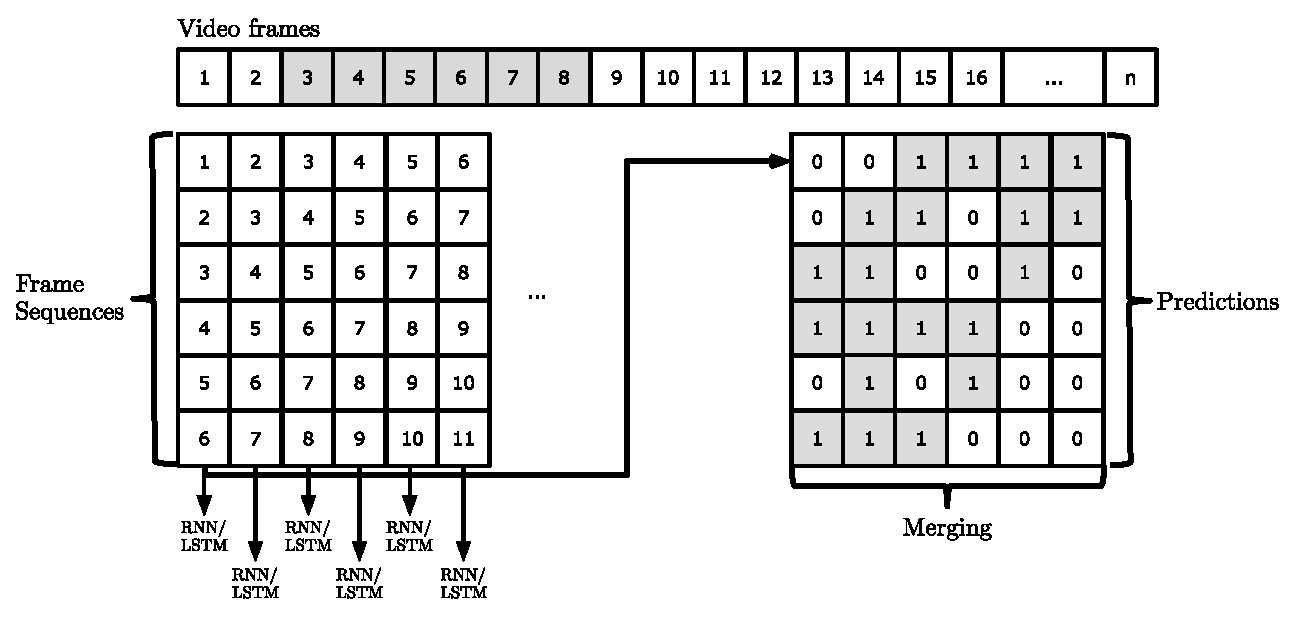
\includegraphics[scale=.7]{images/soft_cut_approach.eps}
	\caption{To classify soft cuts of arbitrary length, we repeatedly test fixed-size frame sequences. In this example we test sequences of size six. Afterwards the predictions given by the RNN/LSTM are merged, so that we have one prediction per frame.}
	\label{fig:soft_cut_approach}
\end{figure}

 has to fit into the batch size.



When classifying a soft cut sequence, the result is one prediction per frame.
We therefore applied several strategies for combining the per-frame result to get one per-sequence result.

\subsection{Evaluation}
\label{sec:hard_cut_evaluation}


